\section{Coarse-grained simulations}

\begin{figure}[ht]
  \begin{centering}
  \adjustbox{minipage=1.3em,valign=t}{\subcaption{}\label{sfig:testa}}%
  \begin{subfigure}[t]{\dimexpr.4\linewidth-1.3em\relax}
  \centering
  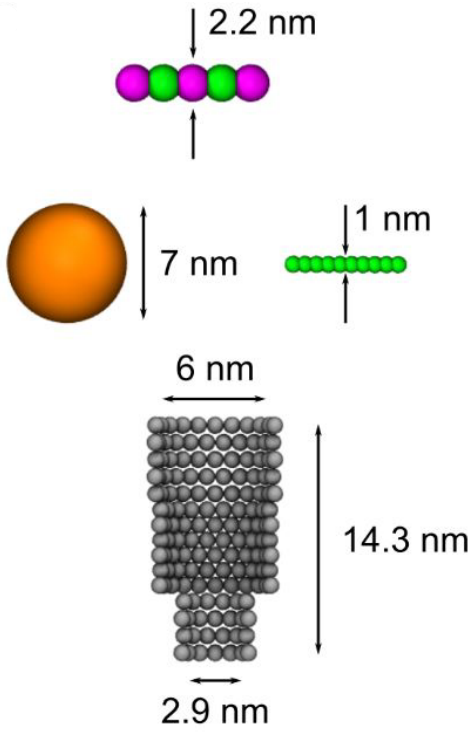
\includegraphics[width=0.9\linewidth,valign=t]{Figures/Stefanos1.png}
  \end{subfigure}%
  \adjustbox{minipage=1.3em,valign=t}{\subcaption{}\label{sfig:testb}}%
  \begin{subfigure}[t]{\dimexpr.5\linewidth-1.3em\relax}
  \centering
  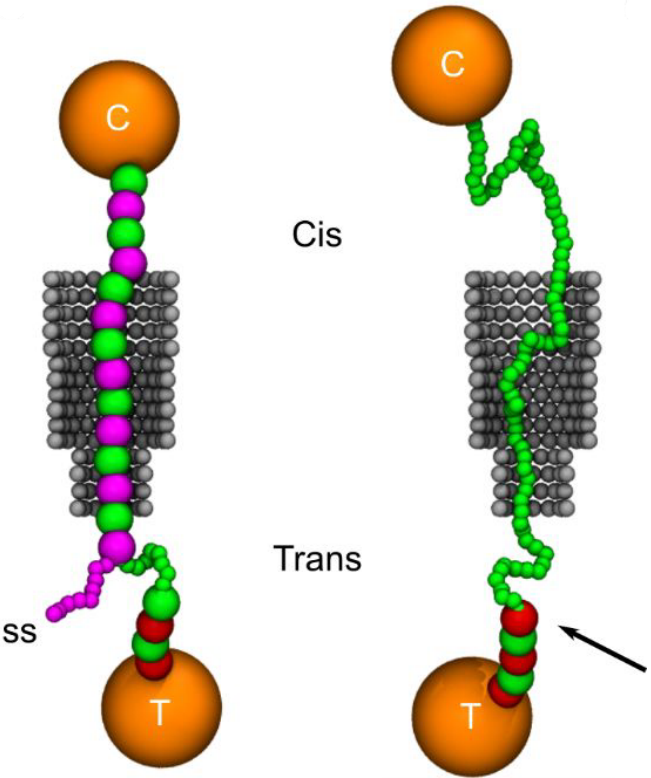
\includegraphics[width=0.9\linewidth,valign=t]{Figures/Stefanos2.png}
  \end{subfigure}
  \caption{This is a figure}
  \label{fig:test}
  \end{centering}
\end{figure}


As is common in simula- tions of coarse-grained models, we use a higher diffusion
coefficient than for physical DNA
